\setchapterpreamble[u]{\margintoc}
\chapter{Carbon Footprints}
\labch{carbon_footprints}

In this chapter I will go over estimating the carbon footprints for each technology.



\section{Direct versus Indirect emissions}

Fossil fuels emit a lot of carbon equivalent gases into the atmosphere. For several generation sources, often referred to as "clean", there is no direct greenhouse gases emissions. This is the case for nuclear, wind, solar, geothermal, biomass and hydroelectricity. However, this does not mean that these technologies do not have a carbon footprint. Indeed, the intensive manufacturing process of the capture elements (wind turbines, solar panels, reactor buildings, \ldots) emit a non negligible amount of $\mathrm{CO_2}$. These emissions are denoted "indirect".

\begin{kaobox}[frametitle=A look at some values]

Let us take a step back and consider how the emissions are usually scored. You will see values given in $gCO_2/kWh$. This is a value one has to be careful with, as a kWh may not be representative of an indirect emission. Solar is usually cited at around 50 g per kWh.

To illustrate this, consider two 5kW solar systems, both built in the exact same way, same plant, same location. Then, use one of these systems in Fairbanks, AK, and the other in Phoenix, AZ. As expected, the performance would be radically different, and we can for example assume the load factor to be 10\% in Fairbanks and 30\% in Phoenix. In that situation, the Alaskan system would generate 4,400 kWh, while the Arizonian system would generate 3 times as much, at 13,000 kWh, over a year.

So, this implies that the Alaskan solar system emits 220 kilograms of $\mathrm{CO_2}$
per year and the Arizonian solar system emits 650 kilograms of $\mathrm{CO_2}$ (still the factor 3).

But this is obviously incorrect, as the emission from solar are indirect, and thus both system emitted the same amount of $\mathrm{CO_2}$, when they were manufactured.

In order to compute the right value, the $gCO_2/kWh$ should be accompanied by a capacity factor value or at least a location, or in other words, the $gCO_2/kW$ should be given.

This issue is true of every means of production where the emissions are indirect and occur during manufacturing.

\end{kaobox}

\begin{figure}[h]
	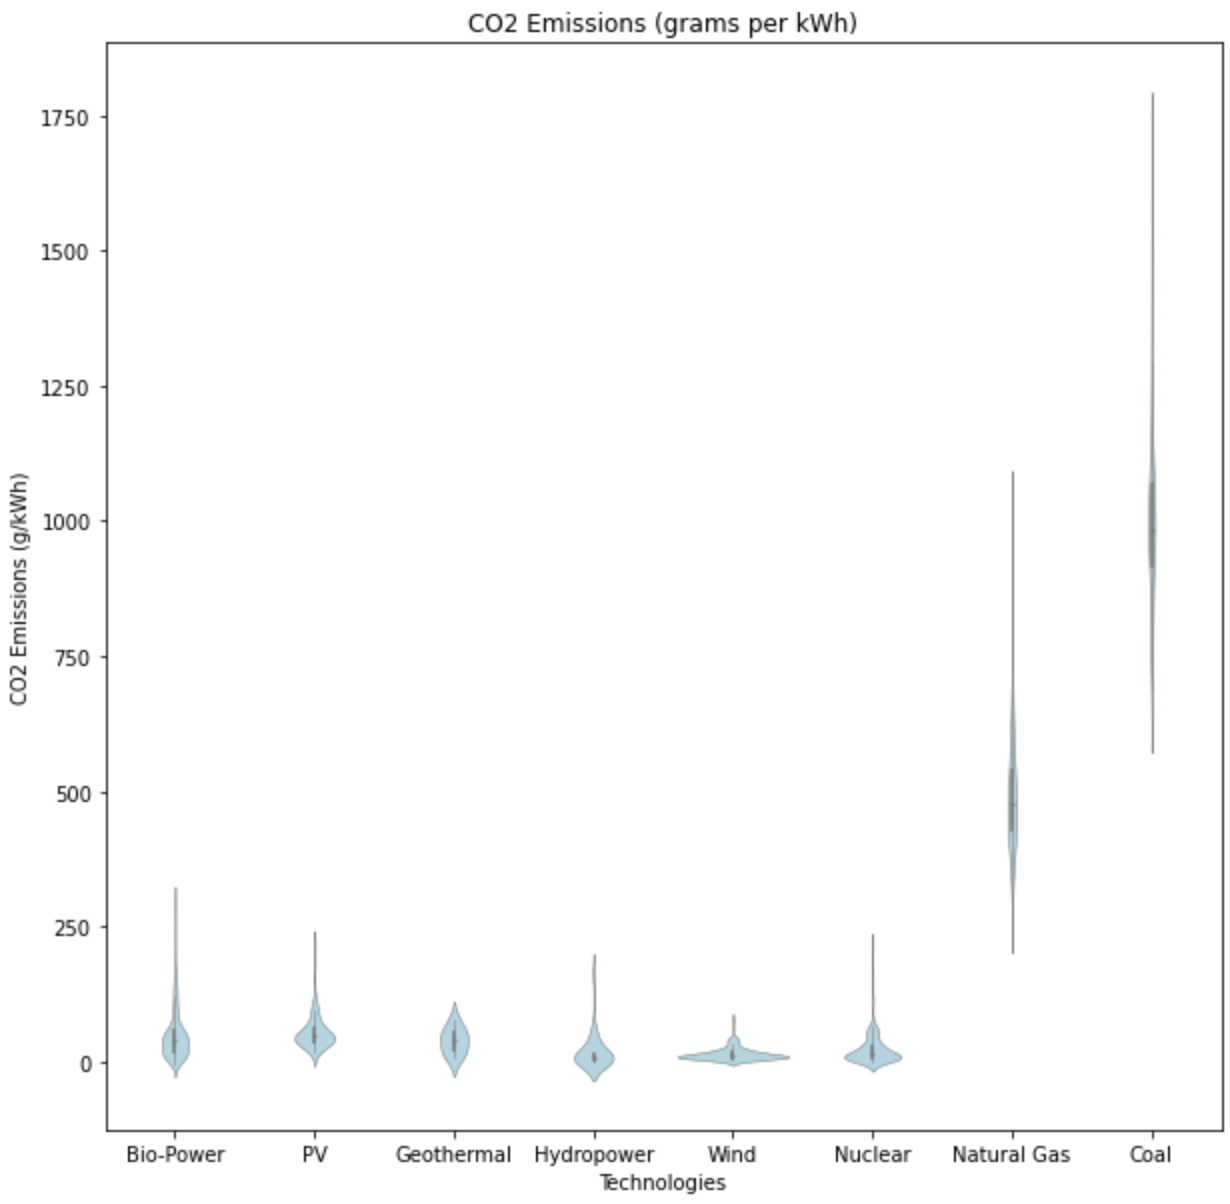
\includegraphics[width=1.0\textwidth]{co2_tech}
	\caption[Adjusted $\mathrm{CO_2}$ Emissions per technology. Keep in mind that this is dependent on capacity factors for the indirect carbon emissions.]{Adjusted $\mathrm{CO_2}$ Emissions per technology. Keep in mind that this is dependent on capacity factors for the indirect carbon emissions.}
	\labfig{co2_tech}
\end{figure}



\section{Technologies footprint}

%SOLAR
%https://www.nature.com/articles/ncomms13728
% In SI, Table 2, we get the CO2 per kW
The indirect $\mathrm{CO_2}$ emissions of solar energy has been shown to be around 1 kg per Wp in the last decade~\sidecite{louwen2016re}. This translates to 1 ton per kWp installed. Another way to think about this is that the manufacturing and installation of your average residential solar roof generates around 5 tons of $\mathrm{CO_2}$. These initial emissions are offset in a few years, depending on the energy mix where the panels are producing.

Wind data is a bit lacking in terms of indirect emissions. Values are often given per location, without explicitly mentioning the assumptions made. We will thus estimate the carbon footprint from harmonized $gCO_2/kWh$ median values\sidecite{dolan2012life}. \vreffig{co2_solar_wind} shows the $\mathrm{CO_2}$ cost for both solar and wind.


\begin{figure}[h]
	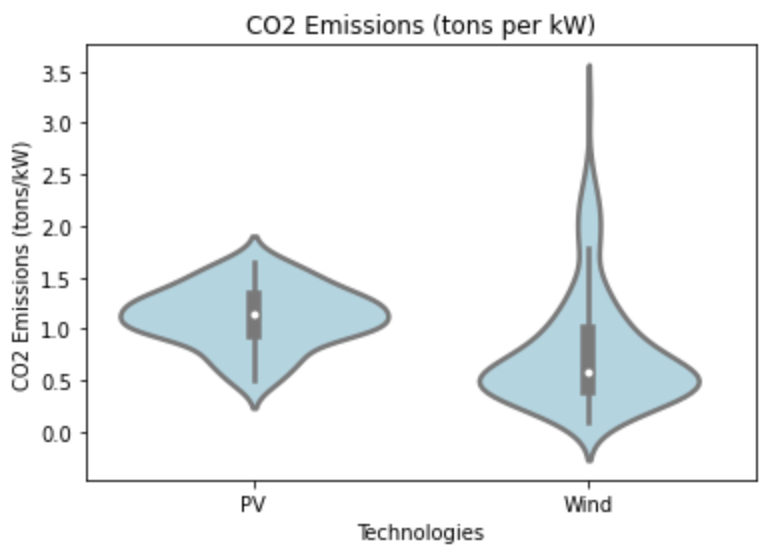
\includegraphics[width=1.0\textwidth]{co2_solar_wind}
	\caption[Adjusted $\mathrm{CO_2}$ Emissions (indirect) for solar and wind power, assuming 30\% capacity factor and 20 years lifetime for wind, and 15\% capacity factor with a 30 years lifetime and a degradation rate of 0.7\% per year for solar.]{Adjusted $\mathrm{CO_2}$ Emissions (indirect) for solar and wind power, assuming 30\% capacity factor and 20 years lifetime for wind, and 15\% capacity factor with a 30 years lifetime and a degradation rate of 0.7\% per year for solar.}
	\labfig{co2_solar_wind}
\end{figure}

An average system of 1 kW installed capacity (capacity factor 30\%, lifetime 20 years) will generate $8760h * 20y * 30\% = 52.5 MWh$. At $11 gCO_2/kWh$, this represents around 0.6 ton of $\mathrm{CO_2}$ per kW.

The batteries impacts in terms of $\mathrm{CO_2}$ emissions are difficult to estimate. To get a reasonable order of magnitude, we use data from~\sidecite{dai2019life,emilsson2019lithium}, and assume a energy mix closer to the Chinese one, where the majority of the battery production happens today. This gives us around 100 kg of $\mathrm{CO_2}$ per kWh capacity installed\sidenote[][]{Note that when it comes to batteries, kWh capacity is not kWh produced, due to the lifetime (number of cycles)}.

Nuclear emissions have been shown to be around a median of 17 $gCO_2/kWh$~\sidecite{warner2012life}. Using the relevant capacity factor of 92\%, and an operational lifetime of 40 years, we can see that each kW of nuclear installed comes with a cost of carbon of approximately 
5 tons per kW, as shown by the median value on~\vreffig{co2_nuclear}. One can note that at first glance, it might seem that nuclear generates 5 to 10 times more $\mathrm{CO_2}$. Be mindful, and recall that our goal here is to get a development carbon cost, meaning that we decorrelate the lifetime and capacity factor (to generate the same energy over time, you need to install a lot more kW of renewable)\sidenote[][-2mm]{Do not compare indirect $gCO_2/kW$ values without care}.

\begin{figure}[h]
	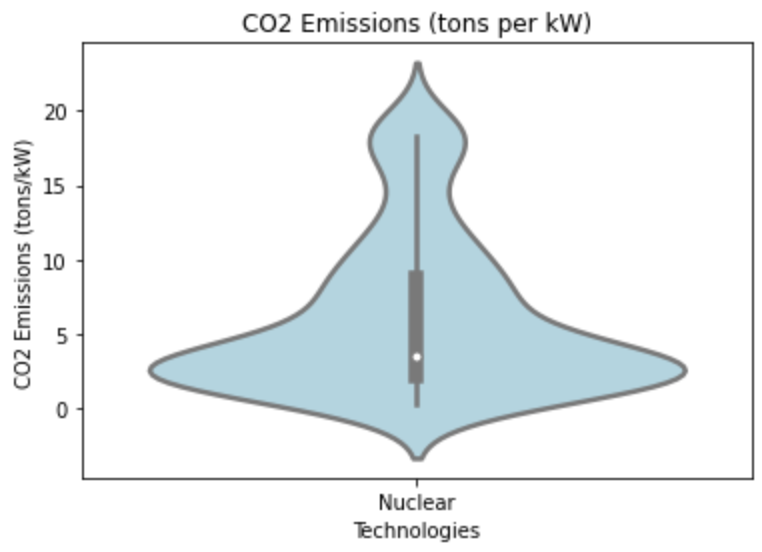
\includegraphics[width=1.0\textwidth]{co2_nuclear}
	\caption[$\mathrm{CO_2}$ Emissions (indirect) for nuclear power.]{$\mathrm{CO_2}$ Emissions (indirect) for nuclear power, assuming a 92\% capacity factor. We can see some high values, resulting from worst case scenarios on the ore type and the enrichment method notably.}
	\labfig{co2_nuclear}
\end{figure}

Natural gas, Coal and Petroleum are clear emitter at production (direct emissions). From the literature, we see that we can approximate natural gas emissions at 475 $gCO_2/kWh$ produced~\sidecite{o2014life}. Coal shows large variability depending on the technology, but a value of 1,000 $gCO_2/kWh$ produced is a good approximation~\sidecite{whitaker2012life}.


\begin{figure}[h]
	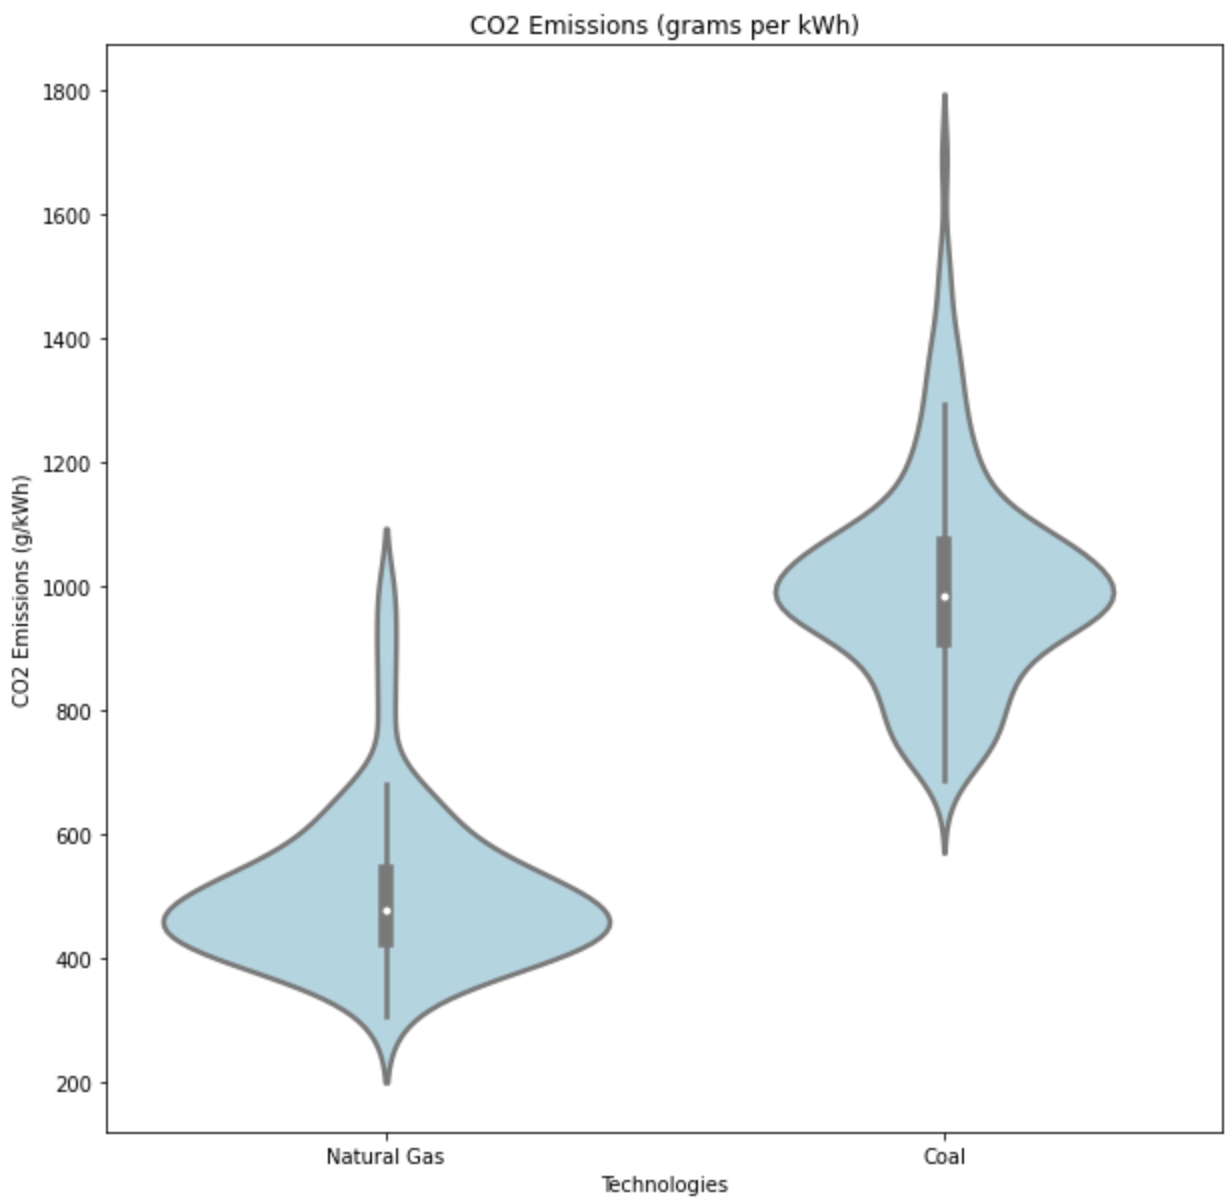
\includegraphics[width=1.0\textwidth]{co2_coal_gas}
	\caption[$\mathrm{CO_2}$ Emissions (direct) for coal and gas power.]{$\mathrm{CO_2}$ Emissions (direct) for coal and gas power.}
	\labfig{co2_coal_gas}
\end{figure}


\begin{kaobox}[frametitle=Indirect emissions\ldots until a cleaner grid?]

It is also important to note that the reason why the indirect emissions of renewable energies manufacturing is so high is due to the current energy mix of the manufacturing places. A solar panel made in China will have a higher $\mathrm{CO_2}$ cost than a solar panel made in Europe, because of the type of energy used in its manufacturing.

As the grid moves toward a cleaner version, the indirect emissions will decrease. At the same time, it is easy to think that the more the grid moves toward a cleaner version, the more the cost and ease of mining and manufacturing could go up.

\end{kaobox}


\begin{table}[ht]
\caption[Carbon emissions per technology]{Carbon emissions per technology}
\labtab{carbon_emissions_technology}
\begin{tabular}{ c c c }
	\toprule
	Technology & Direct (g/kWh) & Indirect (tons/kW) \\
	\midrule
	Natural Gas & 475 & - \\
	Coal & 1000 & - \\
	Nuclear & - & 5000 \\
	Petroleum & 1000 & - \\
	Solar & - & 1 \\
	Wind & - & 0.6 \\
	Hydro & 15 & - \\
	Batteries & - & 100\sidenote[*][-2mm]{kg per kWh capacity} \\
	\bottomrule
\end{tabular}

\end{table}


\section{The Digest}

\begin{kaoboxgreen}[frametitle=Main Takeaways]

\begin{itemize}
\item Normalized by energy produced over their lifetime in an average environment, Nuclear and the renewable energies (Hydroelectricity, Biomass, Solar and Wind) are comparable in terms of emissions, and much lower than fossil fuels.
\item The distinction direct versus indirect emissions is important, as theoretically, almost all indirect emissions could be removed given a clean energy grid.
\item Clean energy emits $\mathrm{CO_2}$ during the manufacturing process, which requires energy from the existing grid, and thus the use of fossil fuel in most cases.
\item Chemical batteries are a non-negligible emitter due to their energy intensive mining and manufacturing process in today's grid. On the other hand, pumped hydro storage has a low carbon footprint.
\end{itemize}
  
\end{kaoboxgreen}


\todo{Appendix: How to read a violin plot?}
